\begin{figure}[htbp]
	\centering
	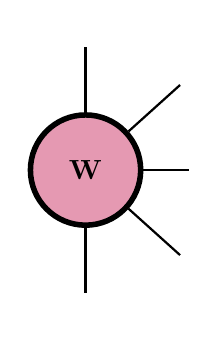
\begin{tikzpicture}[scale=1.2]
		\node[draw, circle, fill=purple!40, minimum size=1.4cm, line width=2pt] (w) at (0,0) {\textbf{W}};
		\draw[thick] (w) -- ++(0,1.3) node[above] {};
		\draw[thick] (w) -- ++(1,0.9);
		\draw[thick] (w) -- ++(1.1,0);
		\draw[thick] (w) -- ++(1,-0.9);
		\draw[thick] (w) -- ++(0,-1.3) node[below] {};


	\end{tikzpicture}
	\caption{The W spider in ZW calculus represents the N-partite W state. The W spider with $N$ legs encodes the superposition where exactly one qubit is in state $|1\rangle$ and the rest are $|0\rangle$, with all permutations equally weighted.}
	\label{fig:zw-w-spider}
\end{figure}
